% SPDX-License-Identifier: BSD-2-Clause
%
% Copyright (C) 2026 embedded brains GmbH & Co. KG
%
% Redistribution and use in source and binary forms, with or without
% modification, are permitted provided that the following conditions
% are met:
% 1. Redistributions of source code must retain the above copyright
%    notice, this list of conditions and the following disclaimer.
% 2. Redistributions in binary form must reproduce the above copyright
%    notice, this list of conditions and the following disclaimer in the
%    documentation and/or other materials provided with the distribution.
%
% THIS SOFTWARE IS PROVIDED BY THE COPYRIGHT HOLDERS AND CONTRIBUTORS "AS IS"
% AND ANY EXPRESS OR IMPLIED WARRANTIES, INCLUDING, BUT NOT LIMITED TO, THE
% IMPLIED WARRANTIES OF MERCHANTABILITY AND FITNESS FOR A PARTICULAR PURPOSE
% ARE DISCLAIMED. IN NO EVENT SHALL THE COPYRIGHT OWNER OR CONTRIBUTORS BE
% LIABLE FOR ANY DIRECT, INDIRECT, INCIDENTAL, SPECIAL, EXEMPLARY, OR
% CONSEQUENTIAL DAMAGES (INCLUDING, BUT NOT LIMITED TO, PROCUREMENT OF
% SUBSTITUTE GOODS OR SERVICES; LOSS OF USE, DATA, OR PROFITS; OR BUSINESS
% INTERRUPTION) HOWEVER CAUSED AND ON ANY THEORY OF LIABILITY, WHETHER IN
% CONTRACT, STRICT LIABILITY, OR TORT (INCLUDING NEGLIGENCE OR OTHERWISE)
% ARISING IN ANY WAY OUT OF THE USE OF THIS SOFTWARE, EVEN IF ADVISED OF THE
% POSSIBILITY OF SUCH DAMAGE.

\documentclass[tikz,border=4pt]{standalone}
\usepackage[T1]{fontenc}
\usepackage[scaled]{helvet}
\renewcommand{\familydefault}{\sfdefault}
\usetikzlibrary{arrows.meta,positioning,fit,backgrounds,shapes.geometric}
\definecolor{ebblue}{HTML}{1F4E79}
\definecolor{boxfill}{HTML}{EAF1F8}
\definecolor{codefill}{HTML}{FFF4E0}
\definecolor{codeline}{HTML}{9C6500}
\definecolor{groupfill}{HTML}{F5F5F5}
\definecolor{flow}{HTML}{404040}
\newcommand{\code}[1]{{\ttfamily\scriptsize #1}}
\begin{document}
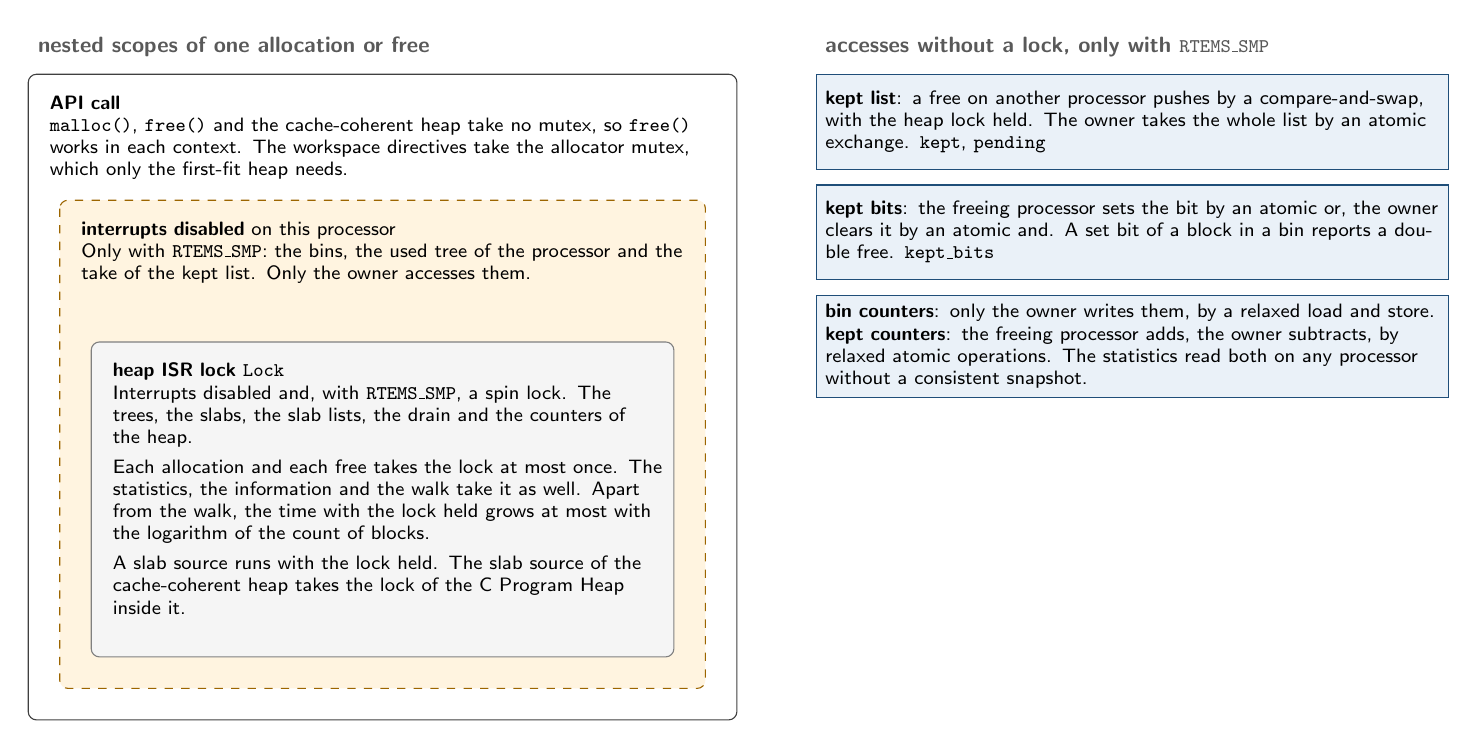
\begin{tikzpicture}[
    font=\small,
    scopebox/.style={rounded corners=3pt, align=left, anchor=north west},
    item/.style={font=\scriptsize, align=left, anchor=north west, text width=#1},
    item/.default=70mm,
    row/.style={draw=ebblue, fill=boxfill, minimum height=12mm, align=left,
      text width=78mm, font=\scriptsize, anchor=north west},
    title/.style={font=\footnotesize\bfseries, text=gray!70!black, anchor=south west}]
  % Nested scopes
  \node[title] at (0,0.1) {nested scopes of one allocation or free};
  \draw[fill=white, draw=flow, rounded corners=3pt] (0,0) rectangle (9.0,-8.2);
  \node[item=86mm] at (0.15,-0.15) {\textbf{API call}\\
    \code{malloc()}, \code{free()} and the cache-coherent heap take no mutex,
    so \code{free()} works in each context.  The workspace directives take the
    allocator mutex, which only the first-fit heap needs.};
  \draw[fill=codefill, draw=codeline, rounded corners=3pt, dashed] (0.4,-1.6) rectangle (8.6,-7.8);
  \node[item=78mm] at (0.55,-1.75) {\textbf{interrupts disabled} on this processor\\
    Only with \code{RTEMS\_SMP}: the bins, the used tree of the processor and
    the take of the kept list.  Only the owner accesses them.};
  \draw[fill=groupfill, draw=gray, rounded corners=3pt] (0.8,-3.4) rectangle (8.2,-7.4);
  \node[item=70mm] at (0.95,-3.55) {\textbf{heap ISR lock} \code{Lock}\\
    Interrupts disabled and, with \code{RTEMS\_SMP}, a spin lock.  The trees,
    the slabs, the slab lists, the drain and the counters of the heap.\\[1mm]
    Each allocation and each free takes the lock at most once.  The statistics,
    the information and the walk take it as well.  Apart from the walk, the time with the
    lock held grows at most with the logarithm of the count of blocks.\\[1mm]
    A slab source runs with the lock held.  The slab source of the
    cache-coherent heap takes the lock of the C Program Heap inside it.};
  % Lock-free accesses
  \node[title] at (10.0,0.1) {accesses without a lock, only with \code{RTEMS\_SMP}};
  \node[row] at (10.0,0) {\textbf{kept list}: a free on another processor pushes by a
    compare-and-swap, with the heap lock held.  The owner takes the whole list
    by an atomic exchange.  \code{kept}, \code{pending}};
  \node[row] at (10.0,-1.4) {\textbf{kept bits}: the freeing processor sets the bit by
    an atomic or, the owner clears it by an atomic and.  A set bit of a block
    in a bin reports a double free.  \code{kept\_bits}};
  \node[row] at (10.0,-2.8) {\textbf{bin counters}: only the owner writes them, by a
    relaxed load and store.  \textbf{kept counters}: the freeing processor adds,
    the owner subtracts, by relaxed atomic operations.  The statistics read both
    on any processor without a consistent snapshot.};
\end{tikzpicture}
\end{document}
